% Speed-strength plane for Marburg outbreaks.
% x = intrinsic growth rate r (per day), y = mean generation interval T_g (days).
% R0 contours use the Wallinga & Lipsitch (2007) relation for an exponentially
% distributed generation interval: R0 = 1 + r*T_g  =>  T_g = (R0 - 1)/r.
% Each outbreak is placed at its estimated r (with 95% CI as a horizontal
% whisker) and spans the assumed pre-2014 serial-interval band 9.3-11.2 days
% (vertical segment); the dot marks the band midpoint. Reading where an
% outbreak's vertical segment crosses the contours gives its R0 range.
%
% Compile with pdflatex (or lualatex) + pgfplots (>= 1.16).
\documentclass[border=3pt]{standalone}
\usepackage{pgfplots}
\pgfplotsset{compat=1.16}
\usepackage{amsmath}

% Okabe-Ito colorblind-safe palette
\definecolor{oiBlack}{RGB}{0,0,0}
\definecolor{oiOrange}{RGB}{230,159,0}
\definecolor{oiSky}{RGB}{86,180,233}
\definecolor{oiGreen}{RGB}{0,158,115}
\definecolor{oiBlue}{RGB}{0,114,178}
\definecolor{oiVermil}{RGB}{213,94,0}

\begin{document}
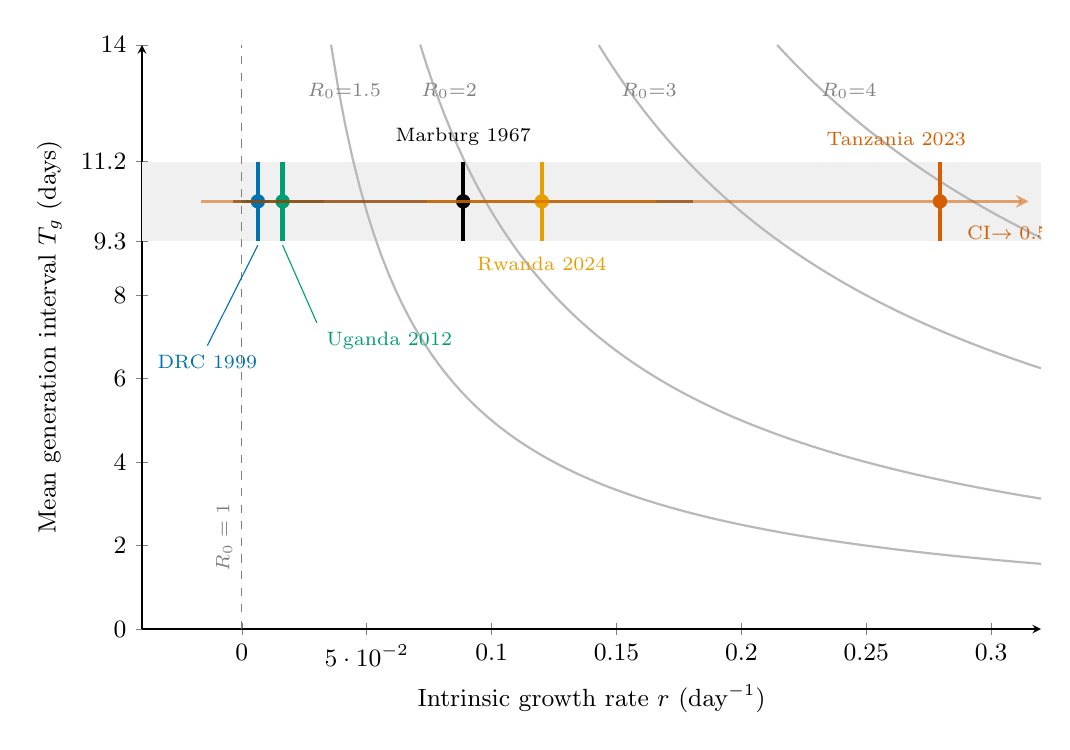
\begin{tikzpicture}
\begin{axis}[
    width=13cm, height=9cm,
    xlabel={Intrinsic growth rate $r$ (day$^{-1}$)},
    ylabel={Mean generation interval $T_g$ (days)},
    xmin=-0.04, xmax=0.32,
    ymin=0, ymax=14,
    axis lines=left,
    xtick={-0.0,0.05,0.10,0.15,0.20,0.25,0.30},
    ytick={0,2,4,6,8,9.3,11.2,14},
    yticklabels={0,2,4,6,8,9.3,11.2,14},
    tick label style={font=\small},
    label style={font=\small},
    clip=true,
]

% ---- serial-interval band 9.3-11.2 days (pre-2014 serial interval) ----
\fill[gray!12] (axis cs:-0.04,9.3) rectangle (axis cs:0.32,11.2);

% ---- R0 contours: T_g = (R0-1)/r ----
\addplot[gray!55,thick,domain=0.0357:0.32,samples=100]{0.5/x};
\addplot[gray!55,thick,domain=0.0714:0.32,samples=100]{1.0/x};
\addplot[gray!55,thick,domain=0.1429:0.32,samples=100]{2.0/x};
\addplot[gray!55,thick,domain=0.2143:0.32,samples=100]{3.0/x};
\node[gray,font=\scriptsize] at (axis cs:0.041,12.9){$R_0{=}1.5$};
\node[gray,font=\scriptsize] at (axis cs:0.083,12.9){$R_0{=}2$};
\node[gray,font=\scriptsize] at (axis cs:0.163,12.9){$R_0{=}3$};
\node[gray,font=\scriptsize] at (axis cs:0.243,12.9){$R_0{=}4$};

% ---- R0 = 1 threshold (r = 0) ----
\draw[gray,dashed] (axis cs:0,0) -- (axis cs:0,14);
\node[gray,font=\scriptsize,rotate=90,anchor=south] at (axis cs:0,2.2){$R_0=1$};

% ---- outbreaks: \obk{r}{r_lo}{r_hi}{color}  draws whisker + band segment + dot ----
\newcommand{\obk}[4]{%
  \draw[#4,opacity=0.55,line width=1pt] (axis cs:#2,10.25) -- (axis cs:#3,10.25);%
  \draw[#4,line width=1.6pt] (axis cs:#1,9.3) -- (axis cs:#1,11.2);%
  \fill[#4] (axis cs:#1,10.25) circle (2.6pt);%
}

% DRC 1999
\obk{0.0064}{0.0015}{0.0113}{oiBlue}
% Uganda 2012
\obk{0.0163}{-0.0003}{0.0329}{oiGreen}
% Marburg 1967
\obk{0.0886}{-0.0036}{0.1808}{oiBlack}
% Rwanda 2024
\obk{0.1201}{0.0743}{0.1658}{oiOrange}
% Tanzania 2023 (all cases) -- upper 95% CI = 0.575 runs off-axis
\draw[oiVermil,opacity=0.55,line width=1pt,-stealth] (axis cs:-0.0164,10.25) -- (axis cs:0.315,10.25);
\draw[oiVermil,line width=1.6pt] (axis cs:0.2795,9.3) -- (axis cs:0.2795,11.2);
\fill[oiVermil] (axis cs:0.2795,10.25) circle (2.6pt);

% ---- labels with leader lines ----
\node[oiBlue,font=\scriptsize,anchor=east] (dLbl) at (axis cs:0.010,6.4){DRC 1999};
\draw[oiBlue,thin] (dLbl.north) -- (axis cs:0.0064,9.2);
\node[oiGreen,font=\scriptsize,anchor=west] (uLbl) at (axis cs:0.030,6.9){Uganda 2012};
\draw[oiGreen,thin] (uLbl.north west) -- (axis cs:0.0163,9.2);
\node[oiBlack,font=\scriptsize,anchor=south] at (axis cs:0.0886,11.35){Marburg 1967};
\node[oiOrange,font=\scriptsize,anchor=north] at (axis cs:0.1201,9.15){Rwanda 2024};
\node[oiVermil,font=\scriptsize,anchor=south] at (axis cs:0.262,11.35){Tanzania 2023};
\node[oiVermil,font=\scriptsize,anchor=west] at (axis cs:0.285,9.5){\,CI$\to0.58$};

\end{axis}
\end{tikzpicture}
\end{document}
